
Now let's address the issue of how to reach a global optima. The algorithm has its specific way of finding an optimal allocation that is derived from evolutionary theory. The idea is that each of the original portfolios are tested, but only the best ones will survive to the next period. These ones will evolve in modifications of the original portfolios and will face the challenge of surviving against a new random generation of portfolios. More specifically the procedure is the following:

\begin{itemize}
	\item First N portfolios are randomly generated. The bigger N the more extensive the search and higher the probability of actually finding an optimal point. This of course comes at a larger expense of optimization time.
	\item Each portfolio is evaluated through the fitness function, so that portfolios can be ranked based on this score.
	\item then a \textbf{selection} step is enforced. Only the best k\% of the portfolios survive, these portfolios will make it to the next optimization round. k is usually in the 20-50\% range, and we will stick to a 30\% value. Moreover, these portfolios are selected to breed a new generation.
	\item The new generation is created through the process of \textbf{mutation}, that means that each portfolio is generated as a little variation of one of the best pre-existing portfolios. An alternative here is \textbf{crossover} that mimics the dynamics of reproduction in the human world. In this case two portfolios would be "mixed" to give birth to a new portfolio. Here we have different alternatives of how to create the crossover, one can just average to portfolios, or select some genes randomly from the two portfolios and so on. For our case we believe mutation works better as we need a faster and simpler method to generate portfolios. Moreover averaging or mixing portfolios would bring us towards almost equally weighted portfolios that we want to avoid since we really want to force our algorithm to search for more extreme and exhotic combinations. 
	\item The remaining part of the set is generated again in a random fashion and the loop starts again.
\end{itemize}

This procedure will hopefully bring to an optimal portfolio. We need to decide how to define an optimal point, or in other words establish when should the optimization terminate. There are many different ways to establish a termination condition, common ones are to stop once a certain performance criteria is reached (i.e a minimum Sharpe Ratio), or to stop the optimization after a fixed amount of time/iterations. Our procedure will be a bit more complex, we will let the evolutionary process continue until a minimum number of iterations will have been done and the improvement in the top portfolios is not that relevant so that it is worth carrying the optimization on. We can see in the following chart a snapshot of an optimization procedure, as we increase the number of iterations the best elements improve their performance until they reach a level where increasing the number of iterations doesn't bring any value to the portfolio.\\

\begin{center}
	\centering
	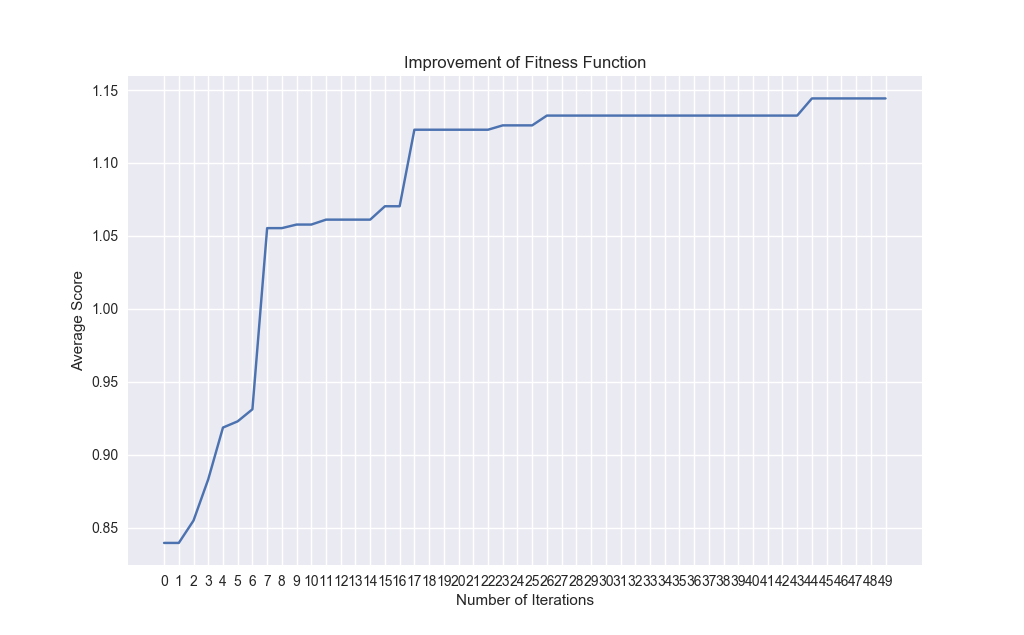
\includegraphics[width=0.6\textwidth]{Genetic_Algo/Fitness_function.png}
	\captionof{figure}{Improvements of portfolio iteration after iteration.}
	\label{Fitness_func}
\end{center}


We now aim to show how this optimization process works in an intuitive and visual way. We consider the optimization process for one date and show the evolution of the various generations of portfolios. We use a nice heatmap where every colour indicates a different "species". At each iteration the species are sorted by score and it is easy to see how as the optimization process goes on some species become dominant and mark the evolution of most of the portfolios.

\todo{Metti foto heatmap optimization}